% Generated by book/tools/notebook_to_tex.py. Do not edit by hand.

\chapter[한국어 BERT 이진 분류 (Korean Binary Classification)]{한국어 BERT 이진 분류 (Korean Binary Classification)}

\label{ch:15}

\markboth{한국어 BERT 이진 분류 (Korean Binary Classification)}{한국어 BERT 이진 분류 (Korean Binary Classification)}

\chaptermeta{15_ko_binary/15_ko_binary.ipynb}{https://colab.research.google.com/github/yoon-gu/neuqes-101/blob/master/15_ko_binary/15_ko_binary.ipynb}{Ch 11의 softmax 이진 분류 셋업을 NSMC와 klue/bert-base로 재현}



\index{1Korean BERT@Korean BERT}

\index{1KLUE BERT@KLUE-BERT}

\index{1klue bert base@klue/bert-base}

\index{1NSMC@NSMC}

\index{1Korean WordPiece@Korean WordPiece}

\index{1CrossEntropyLoss@CrossEntropyLoss}

\index{1single label classification@single\_label\_classification}

\index{1binary classification@binary classification}

\index{0한국어 BERT@한국어 BERT}

\index{0한국어 WordPiece@한국어 WordPiece}

\index{0네이버 영화 리뷰@네이버 영화 리뷰}

\index{0한국어 이진 분류@한국어 이진 분류}

\index{0감성 분류@감성 분류}

\index{0샘플 단위 해석@샘플 단위 해석}

\index{1load dataset@load\_dataset}

\index{1AutoTokenizer@AutoTokenizer}

\index{1AutoModelForSequenceClassification@AutoModelForSequenceClassification}

\index{1num labels 2@num\_labels=2}

\index{1softmax@softmax}

\index{1classification report@classification\_report}

\index{1roc auc score@roc\_auc\_score}

\index{0감성 분석@감성 분석}

\index{0확률 KDE@확률 KDE}

\index{0로짓 분포@로짓 분포}



\section{변화추적표}

\begin{booktable}{15장 변화추적표}{tab:ch15-01}
\begin{adjustbox}{max width=\textwidth}
\begin{tabular}{@{}lllllll@{}}
\toprule
Ch & 모델 & 토크나이저 & 데이터 & Output Head & Activation & Loss \\
\midrule

10 & DistilBERT & WordPiece (영어) & Yelp 이진화 & \inlinecode{Linear(H,\ 1)} & sigmoid & \inlinecode{BCEWithLogitsLoss} \\
11 & DistilBERT & WordPiece (영어) & Yelp 이진화 & \inlinecode{Linear(H,\ 2)} & softmax & \inlinecode{CrossEntropyLoss} \\
\textbf{15 \(\leftarrow\) 여기 (Phase 2 시작)} & \textbf{\inlinecode{klue/bert-base}} & \textbf{WordPiece (한국어)} & \textbf{NSMC (네이버 영화 리뷰)} & \inlinecode{Linear(H,\ 2)} & softmax & \inlinecode{CrossEntropyLoss} \\
16 (다음) & klue/bert-base & WordPiece (한국어) & KLUE-YNAT (뉴스 7분류) & \inlinecode{Linear(H,\ 7)} & softmax & \inlinecode{CrossEntropyLoss} \\
\bottomrule
\end{tabular}
\end{adjustbox}
\end{booktable}

전체 장 표는 \href{https://github.com/yoon-gu/neuqes-101\#챕터별-변화추적표}{루트 README.md}를 참고하세요.



\section{변경점: \ref{ch:11}장 대비}

\begin{booktable}{15장 변경점 요약}{tab:ch15-02}
\begin{adjustbox}{max width=\textwidth}
\begin{tabular}{@{}lll@{}}
\toprule
축 & \ref{ch:11}장 (영어 binary) & \ref{ch:15}장 (한국어 binary) \\
\midrule

\textbf{언어} & 영어 & \textbf{한국어} \\
모델 본체 & \inlinecode{distilbert-base-uncased} (약 66M) & \textbf{\inlinecode{klue/bert-base}} (110M, BERT-base full size) \\
토크나이저 & 영어 WordPiece (vocab 30K) & \textbf{한국어 WordPiece} (vocab 32K) \\
데이터 & Yelp 이진화 (5K샘플 / max\_len 128) & \textbf{NSMC} 5K샘플 / max\_len 128 \\
\inlinecode{num\_labels} & 2 & 2 (그대로) \\
\inlinecode{problem\_type} & \inlinecode{single\_label\_classification} & (그대로) \\
Activation / Loss & softmax / CE & (그대로) \\
라벨 형식 & int 0/1 & int 0/1 (그대로) \\
학습 hyperparams & (epoch=2, lr=2e-5, batch=16, seed=42) & (그대로) \\
\bottomrule
\end{tabular}
\end{adjustbox}
\end{booktable}

\begin{quote}
\textbf{Phase 2 의 \inlinecode{변경점\ 한\ 가지\ 원칙} 변형}: 입문 수준에선 \emph{언어 + 토크나이저 + 데이터} 가 한 묶음으로 같이 변합니다. \emph{모델·loss·셋업이 그대로} 라 가르침은 Phase 1 과 분리해 \emph{한국어 자체의 학습 어려움} 에만 집중할 수 있습니다.
\end{quote}

\subsection{\texorpdfstring{왜 한국어가 영어 BERT 와 \emph{그렇게} 다른가}{왜 한국어가 영어 BERT 와 그렇게 다른가}}

영어 distilbert-base-uncased 토크나이저로 한국어를 처리하면 \emph{처참한} 토큰화가 나옵니다. 영어 vocab 에 한국어 글자가 없어서 \emph{바이트 단위} (\texttt{{[}UNK{]}} 또는 \inlinecode{\#\#} prefix 부스러기) 로 깨집니다. 모델이 학습한 단어 임베딩이 한국어를 못 받아내요.

\textbf{해결}: \emph{한국어 텍스트로 사전학습된} BERT 와 그 토크나이저를 사용. 이 장는 KLUE 연구팀의 \inlinecode{klue/bert-base} --- 한국어 위키 + 뉴스 + 댓글 등으로 사전학습.



\section{손실 노트 --- \ref{ch:11}장 그대로}

\inlinecode{CrossEntropyLoss}. 새로운 점은 없습니다 --- \emph{binary 분류 셋업} 이라 K=2, softmax 후 정답 클래스 확률에 -log.

\begin{equation}
\label{eq:ch15-01}
L = -\frac{1}{N}\sum_{i=1}^{N}\log \hat p_{i, y_i} \quad\text{where}\quad \hat p_{i,k} = \dfrac{e^{z_{i,k}}}{e^{z_{i,0}} + e^{z_{i,1}}}
\end{equation}

식~\eqref{eq:ch15-01}은 이 절에서 사용하는 핵심 관계를 정리한 것입니다.

데이터 분포는 \emph{NSMC 가 거의 완벽 균형} (긍정 \textasciitilde50\%, 부정 \textasciitilde50\%) 이라 random baseline loss = \(\log 2 = 0.693\). 학습 첫 step 에서 loss 가 이 근처면 정상.



\section{토크나이저 노트}

\textbf{\ref{ch:11}장 까지는} \inlinecode{distilbert-base-uncased} (영어 WordPiece) 를 그대로 썼습니다. \textbf{\ref{ch:15}장 부터는} \inlinecode{klue/bert-base} (한국어 WordPiece). 두 토크나이저가 \emph{같은 한국어 문장} 을 어떻게 다르게 쪼개는지가 이 장의 \emph{교훈} 의 절반입니다.

\subsection{직관 --- 같은 문장, 두 토크나이저}

문장: \inlinecode{"이\ 영화\ 정말\ 재미있었어요"}

\begin{booktable}{15장 직관 - 같은 문장, 두 토크나이저 표}{tab:ch15-03}
\begin{adjustbox}{max width=\textwidth}
\begin{tabular}{@{}lll@{}}
\toprule
토크나이저 & 결과 토큰 & 토큰 수 \\
\midrule

\inlinecode{distilbert-base-uncased} (영어) & \texttt{{[}\textquotesingle{}U+110B\textquotesingle{},\ \textquotesingle{}\#\#U+1175\textquotesingle{},\ \textquotesingle{}U+110B\textquotesingle{},\ \textquotesingle{}\#\#U+1167\textquotesingle{},\ \textquotesingle{}\#\#U+11BC\textquotesingle{},\ \textquotesingle{}\#\#U+1112\textquotesingle{},\ \textquotesingle{}\#\#U+116A\textquotesingle{},\ \textquotesingle{}U+110C\textquotesingle{},\ \textquotesingle{}\#\#U+1165\textquotesingle{},\ \textquotesingle{}\#\#U+11BC\textquotesingle{},\ \textquotesingle{}\#\#U+1106\textquotesingle{},\ \textquotesingle{}\#\#U+1161\textquotesingle{},\ \textquotesingle{}\#\#U+11AF\textquotesingle{},\ \textquotesingle{}{[}UNK{]}\textquotesingle{}{]}} 같이 \emph{자모(초·중·종성) 단위} 로 산산조각 (또는 {[}UNK{]} 가득) & 14 \\
\inlinecode{klue/bert-base} (한국어) & \texttt{{[}\textquotesingle{}이\textquotesingle{},\ \textquotesingle{}영화\textquotesingle{},\ \textquotesingle{}정말\textquotesingle{},\ \textquotesingle{}재미있\textquotesingle{},\ \textquotesingle{}\#\#었\textquotesingle{},\ \textquotesingle{}\#\#어요\textquotesingle{}{]}} --- \emph{의미 있는 어휘} 단위 & 6 \\
\bottomrule
\end{tabular}
\end{adjustbox}
\end{booktable}

영어 토크나이저는 한국어를 \emph{낯선 문자열} 로 보고 글자 단위까지 쪼갭니다. 한국어 토크나이저는 \emph{재미있·었·어요} 를 어휘적 의미 단위로 분할 --- 모델이 임베딩을 통해 \emph{의미} 를 잡을 수 있는 형태.

이 비교는 §실습 직전에 \emph{코드로 직접} 확인합니다.

\subsection{한국어 WordPiece 의 특징}

\begin{itemize}
\tightlist
\item
  vocab 32,000 (영어 30K 와 비슷한 규모)
\item
  \emph{어절 단위} 가 아니라 \emph{형태소-비슷한} 서브워드 단위. 예: “재미있었어요” \(\to\) “재미있” + “\#\#었” + “\#\#어요” (어간 + 어미)
\item
  영어처럼 \inlinecode{\#\#} prefix 가 \emph{이전 토큰에 이어지는 부분} 을 표시
\item
  한자·숫자·영어 단어도 vocab 에 포함 (한국어 텍스트엔 흔히 섞여 있음)
\end{itemize}

\subsection{\texorpdfstring{Phase 2 의 토크나이저는 \emph{이 장부터 끝까지} \inlinecode{klue/bert-base} 고정}{Phase 2 의 토크나이저는 이 장부터 끝까지 klue/bert-base 고정}}

\ref{ch:16}장, 17, 18 도 같은 토크나이저. 변하는 건 \emph{데이터·task} 만. 영어 \(\to\) 한국어 전환은 \emph{이 장에서 한 번} 일어나고, 이후엔 한국어 셋업이 표준.



\textbf{baseline VRAM}:



\Needspace{5\baselineskip}
\begin{lstlisting}
!nvidia-smi
\end{lstlisting}

\begin{codeRead}
\textbf{1행}의 \inlinecode{!nvidia-smi}에서는 앞 단계에서 만든 값을 바탕으로 다음 계산을 수행합니다.
\end{codeRead}



\section{토크나이저 비교}

\inlinecode{klue/bert-base} (한국어) 와 \inlinecode{distilbert-base-uncased} (영어) 두 토크나이저로 \emph{같은} 한국어 문장을 처리해 차이를 직접 봅니다.



\Needspace{10\baselineskip}
\begin{lstlisting}
tokenizer_ko = AutoTokenizer.from_pretrained("klue/bert-base")
tokenizer_en = AutoTokenizer.from_pretrained("distilbert-base-uncased")

samples = [
    "이 영화 정말 재미있었어요",
    "별로였어요. 시간 낭비",
    "오랜만에 본 명작이네요!",
]

\end{lstlisting}

\noindent\emph{앞뒤 블록은 모두 텍스트를 모델 입력 텐서로 바꾸는 단계입니다. 길이를 나누어 같은 흐름을 단계별로 확인합니다.}

\Needspace{11\baselineskip}
\begin{lstlisting}[firstnumber=10]
for sent in samples:
    print(f"text: {sent}")
    tok_ko = tokenizer_ko.tokenize(sent)
    tok_en = tokenizer_en.tokenize(sent)
    print(
        f"  klue/bert-base ({len(tok_ko):>2} tokens): "
        f"{tok_ko}"
    )
    print(
        f"  distilbert-en  ({len(tok_en):>2} tokens): "
        f"{tok_en}"
    )
    print()

\end{lstlisting}

\noindent\emph{앞뒤 블록은 모두 텍스트를 모델 입력 텐서로 바꾸는 단계입니다. 길이를 나누어 같은 흐름을 단계별로 확인합니다.}

\Needspace{10\baselineskip}
\begin{lstlisting}[firstnumber=24]
print(
    f"klue/bert-base vocab size:        "
    f"{tokenizer_ko.vocab_size:,}"
)
print(
    f"distilbert-base-uncased vocab:    "
    f"{tokenizer_en.vocab_size:,}"
)
\end{lstlisting}

\begin{codeRead}
\textbf{1행}의 \inlinecode{tokenizer\_ko = ...}에서는 이후 분석에서 사용할 값을 준비합니다. \textbf{2행}의 \inlinecode{tokenizer\_en = ...}에서는 이후 분석에서 사용할 값을 준비합니다. \textbf{4--8행}의 \inlinecode{samples = ...}에서는 이후 분석에서 사용할 값을 준비합니다.
\end{codeRead}

\noindent\textbf{출력.}
\begin{bookoutputbox}
text: 이 영화 정말 재미있었어요
klue/bert-base ( 6 tokens): ['이', '영화', '정말', '재미있', '##었', '##어요']
distilbert-en (14 tokens): ['U+110B', '##U+1175', 'U+110B', '##U+1167', '##...

text: 별로였어요. 시간 낭비
  klue/bert-base ( 6 tokens): ['별로', '##였', '##어요', '.', '시간', '낭비']
distilbert-en (12 tokens): ['[UNK]', '.', 'U+1109', '##U+1175', '##U+1100',...

text: 오랜만에 본 명작이네요!
klue/bert-base ( 8 tokens): ['오랜만', '##에', '본', '명작', '##이', '##네'...
distilbert-en (26 tokens): ['U+110B', '##U+1169', '##U+1105', '##U+1162', '...

klue/bert-base vocab size:        32,000
distilbert-base-uncased vocab:    30,522
\end{bookoutputbox}
\par\vspace{0.9em}



\textbf{관찰}

\begin{itemize}
\tightlist
\item
  한국어 토크나이저는 \emph{어휘적 의미 단위} 로 분할 --- \inlinecode{재미있} + \inlinecode{\#\#었} + \inlinecode{\#\#어요} 처럼 어간·어미를 살림
\item
  영어 토크나이저는 한국어를 \emph{글자 단위} 로 쪼개거나 (\inlinecode{이}, \inlinecode{영}, \inlinecode{\#\#화}) \texttt{{[}UNK{]}} 로 처리 --- 의미를 못 잡음
\item
  vocab 크기는 비슷 (32K vs 30K) 지만 \emph{내용물이 완전히 다름} --- 한국어 vocab 은 한국어 빈도 어휘 32K, 영어 vocab 은 영어 빈도 어휘 30K
\item
  토큰 수도 한국어 토크나이저가 \emph{훨씬 적음} --- 같은 문장이라도 짧은 시퀀스로 표현되어 학습 효율도 좋음
\end{itemize}



\section{데이터 준비}

NSMC = Naver Sentiment Movie Corpus. 한국어 \emph{binary} 감성 분류의 표준 벤치마크. 한 줄짜리 짧은 리뷰 + 긍정(1) / 부정(0) 라벨.

\textbf{원본}: e9t/nsmc GitHub 의 \inlinecode{ratings\_train.txt} / \inlinecode{ratings\_test.txt} TSV. Hugging Face datasets hub 의 nsmc 레포는 \emph{로더 스크립트} 기반이라 최신 datasets 라이브러리에서 deprecated --- 그래서 GitHub raw URL 에서 직접 받습니다.



\section{토큰화 --- \ref{ch:11}장 패턴 그대로, 토크나이저만 한국어로}

\ref{ch:11}장과 \emph{한 줄 차이} --- 토크나이저 인스턴스가 영어 \(\to\) 한국어. 라벨 형식 \inlinecode{int(b)} 도 그대로.



\Needspace{11\baselineskip}
\begin{lstlisting}
tokenizer = tokenizer_ko

def tokenize_fn(batch):
    out = tokenizer(
        batch["text"],
        truncation=True,
        max_length=128,
    )
    out["labels"] = [int(l) for l in batch["label"]]
    return out

train_tok = train_ds.map(tokenize_fn, batched=True).remove_columns(["text", "label"])
eval_tok  = eval_ds.map(tokenize_fn,  batched=True).remove_columns(["text", "label"])

\end{lstlisting}

\noindent\emph{앞 블록은 텍스트를 모델 입력 텐서로 바꾸는 단계입니다. 이어지는 블록에서는 앞에서 만든 중간 값을 다음 계산으로 넘기는 단계로 넘어갑니다.}

\Needspace{11\baselineskip}
\begin{lstlisting}[firstnumber=15]
print(train_tok)
print(
    f"\nFirst sample label: "
    f"{train_tok[0]['labels']}  (int scalar 0=neg / 1=pos)"
)

lens = [len(s) for s in train_tok["input_ids"]]
print(
    f"\nToken length stats — mean: {np.mean(lens):.1f}, median: {np.median(lens):.0f}, max: "
    f"{max(lens)}"
)
\end{lstlisting}

\begin{codeRead}
\textbf{1행}의 \inlinecode{tokenizer = ...}에서는 이후 분석에서 사용할 값을 준비합니다. \textbf{3행}의 \inlinecode{def tokenize\_fn(batch):}에서는 앞 단계에서 만든 값을 바탕으로 다음 계산을 수행합니다. \textbf{4--8행}의 \inlinecode{out = ...}에서는 이후 분석에서 사용할 값을 준비합니다.
\end{codeRead}

\noindent\textbf{출력.}
\begin{bookoutputbox}
Dataset({
    features: ['input_ids', 'token_type_ids', 'attention_mask', 'labels'],
    num_rows: 5000
})

First sample label: 1  (int scalar 0=neg / 1=pos)

Token length stats -- mean: 21.9, median: 17, max: 117
\end{bookoutputbox}
\par\vspace{0.9em}



\section{\texorpdfstring{모델 로드}{모델 로드}}

\ref{ch:11}장에서 \inlinecode{distilbert-base-uncased} 였던 자리만 \inlinecode{klue/bert-base} 로 교체. 분류 헤드 \inlinecode{Linear(H,\ 2)} + \inlinecode{single\_label\_classification} 셋업은 동일.



\Needspace{11\baselineskip}
\begin{lstlisting}
model = AutoModelForSequenceClassification.from_pretrained(
    "klue/bert-base",
    num_labels=2,
    problem_type="single_label_classification",
    id2label={0: "negative", 1: "positive"},
    label2id={"negative": 0, "positive": 1},
)

def param_summary(m):
    total     = sum(p.numel() for p in m.parameters())
    trainable = sum(p.numel() for p in m.parameters() if p.requires_grad)
    return total, trainable

\end{lstlisting}

\noindent\emph{앞뒤 블록은 모두 앞에서 만든 중간 값을 다음 계산으로 넘기는 단계입니다. 길이를 나누어 같은 흐름을 단계별로 확인합니다.}

\Needspace{11\baselineskip}
\begin{lstlisting}[firstnumber=14]
total, trainable = param_summary(model)
print(
    f"Parameters:           {total:>13,}  ("
    f"{total/1e6:.1f} M)"
)
print(
    f"Trainable parameters: {trainable:>13,}  ("
    f"{trainable/total:.1%})"
)
print(f"Classifier:           {model.classifier}")
print(
    f"problem_type:         "
    f"{model.config.problem_type}"
)
print(f"hidden size H:        {model.config.hidden_size}")
print(
\end{lstlisting}

\noindent\emph{앞뒤 블록은 모두 앞에서 만든 중간 값을 다음 계산으로 넘기는 단계입니다. 길이를 나누어 같은 흐름을 단계별로 확인합니다.}

\Needspace{5\baselineskip}
\begin{lstlisting}[firstnumber=30]
    f"vocab size V:         "
    f"{model.config.vocab_size:,}"
)
\end{lstlisting}

\noindent\textbf{출력.}
\begin{bookoutputbox}
Key                                        | Status     | 
-------------------------------------------+------------+-
classifier.bias                            | MISSING    | 
classifier.weight                          | MISSING    | 

- MISSING: those params were newly initialized because missing from the che...
Parameters:             110,618,882  (110.6 M)
Trainable parameters:   110,618,882  (100.0%)
Classifier:           Linear(in_features=768, out_features=2, bias=True)
problem_type:         single_label_classification
hidden size H:        768
vocab size V:         32,000
\end{bookoutputbox}
\par\vspace{0.9em}



\textbf{파라미터 수 비교 --- \ref{ch:11}장 vs \ref{ch:15}장}

\begin{booktable}{15장 모델 로드 표}{tab:ch15-04}
\begin{adjustbox}{max width=\textwidth}
\begin{tabular}{@{}lll@{}}
\toprule
& \ref{ch:11}장 (\inlinecode{distilbert-base-uncased}) & \ref{ch:15}장 (\inlinecode{klue/bert-base}) \\
\midrule

Layer 수 & 6 & 12 (BERT-base full) \\
Hidden size H & 768 & 768 \\
총 파라미터 & 약 67M (헤드 포함) & \textbf{110M} \\
\bottomrule
\end{tabular}
\end{adjustbox}
\end{booktable}

\inlinecode{klue/bert-base} 는 BERT-base 풀 사이즈 (12 레이어). DistilBERT 는 그 절반(6 레이어)으로 distill 한 \emph{경량} 모델. 그래서 같은 5K 샘플 학습이 \emph{약 1.5-2 배} 시간이 더 걸립니다.



\Needspace{5\baselineskip}
\begin{lstlisting}
!nvidia-smi
\end{lstlisting}



\section{학습}

\inlinecode{compute\_metrics} 도 binary 분류용 그대로.



\Needspace{11\baselineskip}
\begin{lstlisting}
def compute_metrics(eval_pred):
    logits, labels = eval_pred

    exp = np.exp(logits - logits.max(axis=1, keepdims=True))
    probs_full = exp / exp.sum(axis=1, keepdims=True)
    probs = probs_full[:, 1]
    preds = probs_full.argmax(axis=1)

    p, r, f1, _ = precision_recall_fscore_support(
        labels,
        preds,
        average="binary",
        zero_division=0,
    )
    return {
        "accuracy":  float(accuracy_score(labels, preds)),
\end{lstlisting}

\noindent\emph{앞 블록은 예측 결과를 지표와 표로 요약하는 단계입니다. 이어지는 블록에서는 앞에서 만든 중간 값을 다음 계산으로 넘기는 단계로 넘어갑니다.}

\Needspace{7\baselineskip}
\begin{lstlisting}[firstnumber=17]
        "precision": float(p),
        "recall":    float(r),
        "f1":        float(f1),
        "auc":       float(roc_auc_score(labels, probs)),
    }
\end{lstlisting}



\Needspace{5\baselineskip}
\begin{lstlisting}
!nvidia-smi
\end{lstlisting}



\section{평가}

\ref{ch:11}장의 평가 패턴 그대로 --- 2차원 logit 에서 softmax \(\to\) 클래스 1 확률 추출, 1차원 logit z = z\_1 - z\_0 도 같이 만들어 시각화 호환.



\Needspace{10\baselineskip}
\begin{lstlisting}
preds_output = trainer.predict(eval_tok)
logits2 = preds_output.predictions
labels  = preds_output.label_ids.astype(int)

exp = np.exp(logits2 - logits2.max(axis=1, keepdims=True))
probs_full = exp / exp.sum(axis=1, keepdims=True)
probs = probs_full[:, 1]
logits = logits2[:, 1] - logits2[:, 0]

\end{lstlisting}

\noindent\emph{앞 블록은 학습 설정을 만들고 학습 루프를 실행하는 단계입니다. 이어지는 블록에서는 모델 출력을 확률이나 예측값으로 바꾸는 단계로 넘어갑니다.}

\Needspace{11\baselineskip}
\begin{lstlisting}[firstnumber=10]
print(f"logits2 (raw)  shape: {logits2.shape}")
print(
    f"logit z = z1-z0 range: [{logits.min():.2f}, "
    f"{logits.max():.2f}]"
)
print(
    f"prob range:           [{probs.min():.4f}, "
    f"{probs.max():.4f}]"
)
print(
    f"positive prediction rate (prob >= 0.5): "
    f"{(probs >= 0.5).mean():.1%}"
)
\end{lstlisting}

\begin{codeRead}
\textbf{1행}의 \inlinecode{preds\_output = ...}에서는 학습된 모델로 최종 예측값을 만듭니다. \textbf{2행}의 \inlinecode{logits2 = ...}에서는 이후 분석에서 사용할 값을 준비합니다. \textbf{3행}의 \inlinecode{labels = ...}에서는 이후 분석에서 사용할 값을 준비합니다.
\end{codeRead}



\Needspace{7\baselineskip}
\begin{lstlisting}
print(classification_report(
    labels, probs_full.argmax(axis=1),
    target_names=["negative", "positive"],
    digits=4,
))
\end{lstlisting}

\noindent\textbf{출력.}
\begin{bookoutputbox}
precision    recall  f1-score   support

    negative     0.8516    0.8822    0.8667       501
    positive     0.8773    0.8457    0.8612       499

    accuracy                         0.8640      1000
   macro avg     0.8645    0.8640    0.8639      1000
weighted avg     0.8645    0.8640    0.8640      1000
\end{bookoutputbox}
\par\vspace{0.9em}



\subsection{확률 공간 KDE (\ref{ch:11}장과 동일 패턴)}



\compactCodeOmitted{숫자 결과를 그림으로 확인하는 단계}

\begin{bookfigurelabel}[H]{NSMC 이진 분류의 positive 확률 분포}{fig:ch15-probability-kde}
\centering
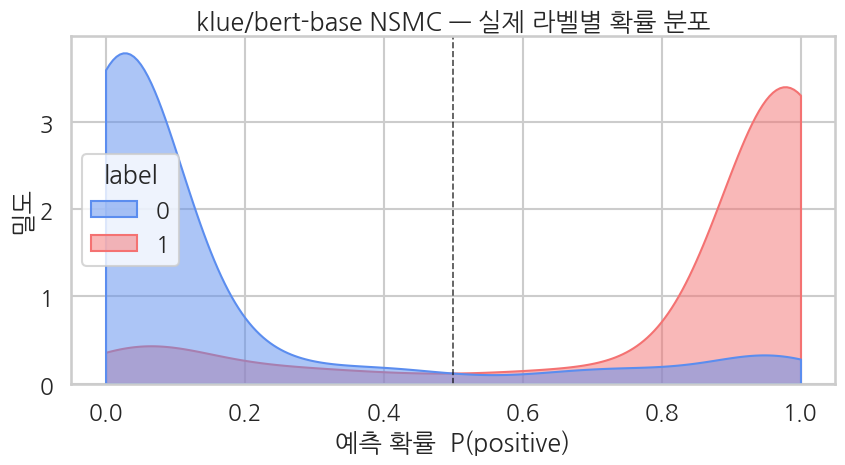
\includegraphics[width=0.88\linewidth]{assets/figures/ch15_probability_kde.png}
\end{bookfigurelabel}

\textbf{그림 읽기} --- 그림~\ref{fig:ch15-probability-kde}에서 다음 내용을 확인합니다: NSMC 이진 분류의 positive 확률 분포. 실행된 노트북에서 저장된 최신 plot 출력이므로, 코드에서 계산한 값이 어떤 평가 지점으로 이어지는지 바로 확인할 수 있습니다.



\subsection{로짓 분포}



\compactCodeOmitted{숫자 결과를 그림으로 확인하는 단계}

\begin{bookfigurelabel}[H]{NSMC 이진 분류의 logit 차이 분포}{fig:ch15-logit-kde}
\centering
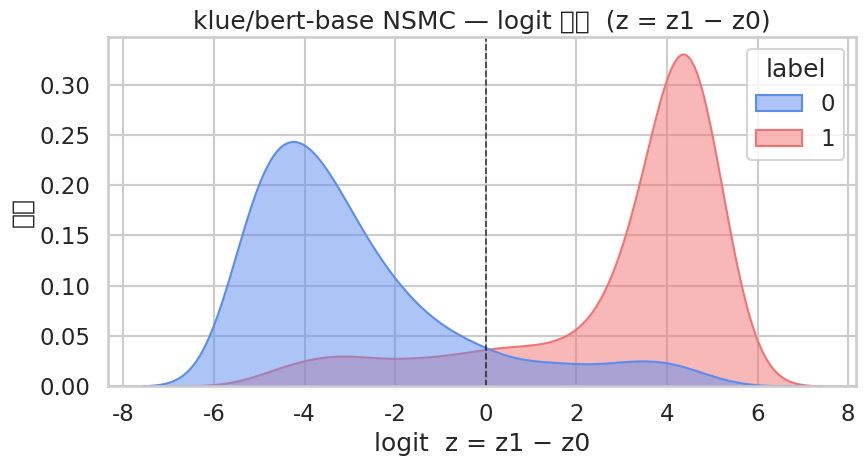
\includegraphics[width=0.88\linewidth]{assets/figures/ch15_logit_kde.png}
\end{bookfigurelabel}

\textbf{그림 읽기} --- 그림~\ref{fig:ch15-logit-kde}에서 다음 내용을 확인합니다: NSMC 이진 분류의 logit 차이 분포. 실행된 노트북에서 저장된 최신 plot 출력이므로, 코드에서 계산한 값이 어떤 평가 지점으로 이어지는지 바로 확인할 수 있습니다.



\textbf{해석}

\begin{itemize}
\tightlist
\item
  두 KDE 가 잘 분리되면 모델이 한국어 감성을 학습한 것. NSMC 는 짧은 한 줄 리뷰라 정보가 적어 영어 Yelp 보다 \emph{조금 더 어려운} 데이터.
\item
  보통 NSMC 5K 샘플 + 2 에폭이면 accuracy 85-88\% 정도. 90\%+ 가 목표면 학습 데이터를 30K 이상으로 늘려야 함.
\end{itemize}



\subsection{샘플 단위 해석}

평가 데이터에서 \emph{모델이 가장 자신 있는} 샘플과 \emph{가장 망설이는} 샘플을 골라 직접 읽어봅니다. 짧은 한국어 리뷰가 모델 입장에서 어떻게 보이는지 감을 잡습니다.



\Needspace{11\baselineskip}
\begin{lstlisting}
texts = list(df_eval.assign(text=eval_ds["text"])["text"]) if "text" in eval_ds.column_names else list(eval_ds["text"])

idx_top_pos    = int(np.argmax(probs))
idx_top_neg    = int(np.argmin(probs))
idx_uncertain  = int(np.argmin(np.abs(probs - 0.5)))

samples = [
    ("most confident positive", idx_top_pos),
    ("most confident negative", idx_top_neg),
    ("most uncertain (prob ~ 0.5)", idx_uncertain),
]

\end{lstlisting}

\noindent\emph{앞 블록은 앞에서 만든 중간 값을 다음 계산으로 넘기는 단계입니다. 이어지는 블록에서는 모델 출력을 확률이나 예측값으로 바꾸는 단계로 넘어갑니다.}

\Needspace{11\baselineskip}
\begin{lstlisting}[firstnumber=13]
for label_str, idx in samples:
    print("=" * 78)
    print(f"sample #{idx}  ({label_str})")
    print("=" * 78)
    print(f"text:        {texts[idx]}")
    print(
        f"true label:  {labels[idx]}  ("
        f"{'positive' if labels[idx] == 1 else 'negative'})"
    )
    print(f"prob(pos):   {probs[idx]:.4f}")
    print(f"logit z:     {logits[idx]:+.2f}")
    pred_label = int(probs[idx] >= 0.5)
    pred_str = "positive" if pred_label == 1 else "negative"
    match = "OK" if pred_label == labels[idx] else "X"
    print(
        f"prediction:  {pred_label} ({pred_str})    match: "
\end{lstlisting}

\noindent\emph{앞 블록은 모델 출력을 확률이나 예측값으로 바꾸는 단계입니다. 이어지는 블록에서는 앞에서 만든 중간 값을 다음 계산으로 넘기는 단계로 넘어갑니다.}

\Needspace{5\baselineskip}
\begin{lstlisting}[firstnumber=29]
        f"{match}"
    )
    print()
\end{lstlisting}

\noindent\textbf{출력.}
\begin{bookoutputbox}
==============================================================================
sample #580  (most confident positive)
==============================================================================
text: 아 최고.. 지금 수능 끝나고 보고 있어요ㅠㅠ 현실적인 30대의 사랑이야기~
true label:  1  (positive)
prob(pos):   0.9944
logit z:     +5.19
prediction:  1 (positive)    match: OK

==============================================================================
sample #169  (most confident negative)
==============================================================================
text:        한마디로노잼 재미없음
true label:  0  (negative)
prob(pos):   0.0033
logit z:     -5.71
...
\end{bookoutputbox}
\par\vspace{0.9em}



\textbf{관찰 포인트}

\begin{itemize}
\tightlist
\item
  \emph{가장 자신있는} 샘플들은 보통 \emph{명확한 감성 표현} 이 들어 있음 (\inlinecode{"인생\ 영화"}, \inlinecode{"시간\ 아까움"} 같은). 모델이 그런 시그널 단어 + 문맥을 잘 잡았다는 신호.
\item
  \emph{망설이는 샘플 (prob \(\approx\) 0.5)} 은 \emph{모호하거나 짧거나 반어} 인 경우. NSMC 에는 \inlinecode{"음..."}, \inlinecode{"글쎄요"} 같은 한 두 글자 리뷰도 있어 모델 입장에선 정보 부족.
\item
  자신 있는 \emph{오답} (틀렸는데 prob 가 0.9+) 이면 \emph{반어법} (\inlinecode{"이게\ 영화냐\ ㅎㅎ"} 형태) 이거나 라벨 노이즈. NSMC 에 라벨 오류가 \textasciitilde3-5\% 있다고 알려져 있음.
\end{itemize}



\section{이 장에 등장한 라이브러리·함수}

\begin{booktable}{15장 새로 등장한 라이브러리}{tab:ch15-05}
\begin{adjustbox}{max width=\textwidth}
\begin{tabular}{@{}lll@{}}
\toprule
이름 & 한 줄 설명 & 다음 장에서 \\
\midrule

\inlinecode{AutoTokenizer.from\_pretrained("klue/bert-base")} & 한국어 BERT-base 토크나이저 (vocab 32K) & \ref{ch:16}--\ref{ch:18}장 모두 같은 토크나이저 \\
\inlinecode{AutoModelForSequenceClassification.from\_pretrained("klue/bert-base",\ ...)} & 한국어 BERT-base + 분류 헤드 & \ref{ch:16}--\ref{ch:18}장 모델 본체 \\
\texttt{pandas.read\_csv(URL,\ sep=“\textbackslash{}t”)} & GitHub raw TSV 직접 다운로드 & NSMC 외에도 자주 쓰는 패턴 \\
\inlinecode{Dataset.from\_pandas(df)} & pandas DataFrame \(\to\) datasets.Dataset 변환 & 외부 데이터를 transformers 파이프라인에 연결 \\
\bottomrule
\end{tabular}
\end{adjustbox}
\end{booktable}



\section{체크포인트 질문}

\begin{enumerate}
\def\labelenumi{\arabic{enumi}.}
\tightlist
\item
  같은 한국어 문장을 영어 토크나이저 (\inlinecode{distilbert-base-uncased}) 와 한국어 토크나이저 (\inlinecode{klue/bert-base}) 로 토큰화한 결과가 왜 \emph{그렇게} 다른가요? vocab 의 어떤 차이가 핵심인가요?
\item
  NSMC 가 영어 Yelp 와 비교해 \emph{왜 더 어려운} 데이터인지 두 가지만 들어보세요.
\item
  \inlinecode{klue/bert-base} 의 파라미터 수가 110M, DistilBERT 가 67M 인데 정확도 차이가 \emph{극적이지 않은} 이유는?
\item
  \ref{ch:11}장과 \ref{ch:15}장 사이에 \emph{셋업 코드 자체} 가 거의 똑같은데도 장를 분리한 이유는?
\end{enumerate}



\section{FAQ}

\begin{faqBox}{Q1. (실무) 한국어 BERT 모델로 \inlinecode{klue/bert-base} 외에 어떤 선택지가 있나요?}

\textbf{기본 (입문)}:

\begin{itemize}
\tightlist
\item
  \inlinecode{klue/bert-base} (110M) --- 이 장. KLUE 벤치마크와 함께 공개, 한국어 표준.
\item
  \inlinecode{klue/roberta-base} (110M) --- RoBERTa 변형, NSP 없이 학습. 보통 KLUE 벤치마크에서 BERT 보다 약간 좋음.
\end{itemize}

\textbf{경량화 (속도/메모리)}:

\begin{itemize}
\tightlist
\item
  \inlinecode{monologg/kobert} (90M) --- 초기 한국어 BERT, 입력 vocab 이 작음.
\item
  \inlinecode{monologg/distilkobert} (\textasciitilde28M) --- DistilBERT 한국어 버전. 로컬 inference 빠름.
\end{itemize}

\textbf{대형 (정확도)}:

\begin{itemize}
\tightlist
\item
  \inlinecode{klue/roberta-large} (340M) --- 메모리·시간 충분하면.
\item
  \inlinecode{kykim/bert-kor-base} (110M) --- 다른 사전학습 코퍼스 (대화체에 강함).
\end{itemize}

\textbf{선택 기준}:

\begin{itemize}
\tightlist
\item
  \emph{입문/실험}: klue/bert-base
\item
  \emph{프로덕션 + 속도}: distilkobert
\item
  \emph{최고 정확도}: klue/roberta-large 또는 deberta-v3-large 한국어 변형
\end{itemize}

\end{faqBox}



\begin{faqBox}{Q4. (실무) \inlinecode{klue/bert-base} 가 NSMC 학습에 \emph{왜 잘 들어맞나}?}

KLUE 사전학습 코퍼스에 \emph{한국어 영화 리뷰 + 댓글} 이 포함되어 있어 NSMC 의 \emph{짧고 구어체} 인 문장 분포를 BERT 가 이미 익힌 상태입니다. 위키만으로 사전학습된 한국어 모델은 NSMC 같은 \emph{비-격식} 텍스트에 약함.

도메인이 \emph{격식체 문서} (법률·특허·논문) 면 \inlinecode{kpfbert/bert-base-korean-legal-news} 같은 도메인 특화 모델이 더 나을 수 있음.

\end{faqBox}


\begin{faqBox}{Q6. (실무) 한국어 sentiment task 에서 prediction confidence 가 0.5 근처에 몰리는 샘플들은 보통 어떤 케이스?}

세 가지 패턴:

\begin{enumerate}
\def\labelenumi{\arabic{enumi}.}
\tightlist
\item
  \textbf{반어/풍자} --- \inlinecode{"이걸\ 영화라고\ 만든\ 거야\ ㅎㅎ"} 처럼 \emph{문자적 의미와 반대} 의 sentiment. 모델이 표면 단어 (\inlinecode{영화}, \inlinecode{만든}) 와 부정 신호 (\inlinecode{ㅎㅎ} 비웃음) 사이에서 갈팡질팡.
\item
  \textbf{모호한 평가} --- \inlinecode{"단순히\ 그랬음"}, \inlinecode{"볼만함"} 같은 \emph{중립에 가까운} 표현. NSMC 라벨 자체가 binary 라 양쪽 다 가능.
\item
  \textbf{너무 짧음} --- \inlinecode{"음..."}, \inlinecode{"글쎄"} 같은 1-2 글자 리뷰. 모델이 판단할 정보 부족.
\end{enumerate}

운영 환경에선 prob ∈ {[}0.4, 0.6{]} 샘플들을 \emph{human review} 로 보내는 패턴이 흔함 (active learning).
\end{faqBox}



\compactFAQMore{3}

\section{오류 실험 (선택)}

다음 코드를 돌려보면 어떤 결과가 나올까요?

\Needspace{6\baselineskip}
\begin{lstlisting}
tokenizer_wrong = AutoTokenizer.from_pretrained("distilbert-base-uncased")
model_wrong = AutoModelForSequenceClassification.from_pretrained(
    "distilbert-base-uncased", num_labels=2,
)
\end{lstlisting}

힌트: \emph{코드는 에러 없이 돌아가지만} accuracy 가 50\% (random baseline) 근처에 머뭅니다. 영어 vocab 이 한국어를 \emph{이해할 수 없는 부스러기} 로 토큰화해 모델이 학습할 신호가 거의 없음. \emph{Phase 2 의 핵심 교훈} --- 한국어엔 \emph{반드시} 한국어 토크나이저 + 한국어 사전학습 모델.



\begin{previewBox}{미리보기: 다음 장}

\textbf{\ref{ch:16}장. 한국어 BERT 다중 클래스 분류 (Korean Multi-class Classification)}

\begin{itemize}
\tightlist
\item
  같은 \inlinecode{klue/bert-base}, 같은 토크나이저, 같은 학습 hyperparams
\item
  변하는 축: \emph{task 차원} (binary K=2 \(\to\) multi-class K=7)
\item
  데이터: KLUE-YNAT (뉴스 헤드라인 7분류 --- 정치/경제/사회/문화/세계/IT/스포츠)
\item
  \ref{ch:12}장의 한국어 버전. 같은 셋업이 K=2·5·7 어디서나 똑같이 동작하는 \emph{일관성} 확인
\end{itemize}

\begin{quote}
\textbf{Phase 2 흐름}: Binary (\ref{ch:15}장) \(\to\) Multi-class (\ref{ch:16}장) \(\to\) Multi-label (\ref{ch:17}장) \(\to\) Auxiliary (\ref{ch:18}장). 토크나이저·모델·hyperparams 가 \emph{Phase 2 안에서는 고정} 이고, \emph{task 만} 바뀝니다.
\end{quote}
\end{previewBox}